\documentclass[border=3pt,tikz]{standalone}
\usepackage{tikz}
\usepackage{listofitems} % for \readlist to create arrays
\tikzstyle{mynode}=[thick,draw=blue,fill=blue!20,circle,minimum size=22]
\begin{document}
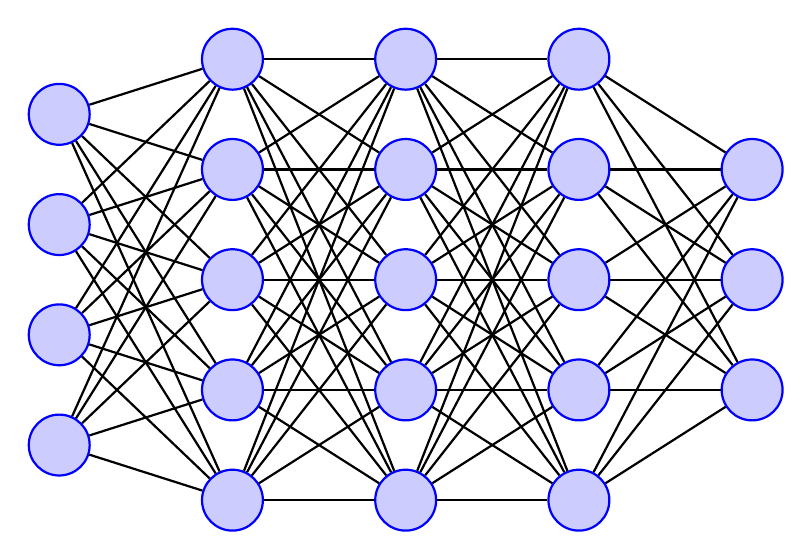
\begin{tikzpicture}[x=2.2cm,y=1.4cm]
  \readlist\Nnod{4,5,5,5,3} % number of nodes per layer
  % \Nnodlen = length of \Nnod (i.e. total number of layers)
  % \Nnod[1] = element (number of nodes) at index 1
  \foreachitem \N \in \Nnod{ % loop over layers
    % \N     = current element in this iteration (i.e. number of nodes for this layer)
    % \Ncnt  = index of current layer in this iteration
    \foreach \i [evaluate={\x=\Ncnt; \y=\N/2-\i+0.5; \prev=int(\Ncnt-1);}] in {1,...,\N}{ % loop over nodes
      \node[mynode] (N\Ncnt-\i) at (\x,\y) {};
      \ifnum\Ncnt>1 % connect to previous layer
        \foreach \j in {1,...,\Nnod[\prev]}{ % loop over nodes in previous layer
          \draw[thick] (N\prev-\j) -- (N\Ncnt-\i); % connect arrows directly
        }
      \fi % else: nothing to connect first layer
    }
  }
\end{tikzpicture}



% \begin{tikzpicture}[x=2.2cm,y=1.4cm]
%   \foreach \N [count=\lay,remember={\N as \Nprev (initially 0);}]
%                in {4,5,5,5,3}{ % loop over layers
%     \foreach \i [evaluate={\y=\N/2-\i; \x=\lay; \prev=int(\lay-1);}]
%                  in {1,...,\N}{ % loop over nodes
%       \node[mynode] (N\lay-\i) at (\x,\y) {};
%       \ifnum\Nprev>0 % connect to previous layer
%         \foreach \j in {1,...,\Nprev}{ % loop over nodes in previous layer
%           \draw[thick] (N\prev-\j) -- (N\lay-\i);
%         }
%       \fi
%     }
%   }
% \end{tikzpicture}
\end{document}
